\clearpage
\section{Results}

\subsection{Model Results}

\paragraph{Classical models.} \tref{tab:classical} compares the final version of each classical model under identical folds and the same test set; \fref{fig:classical} shows the spread across the 50 cross-validation folds and the test confusion matrices.

\begin{table}[H]
\centering
\caption{Final classical models on DS1. CV columns: mean of 10~$\times$~5-fold stratified cross-validation on the 320 training patients. Test columns: one evaluation on the 80 held-out patients (50 CKD, 30 not CKD).}
\label{tab:classical}
\small
\begin{tabular}{lcccccc}
\toprule
 & \multicolumn{3}{c}{Repeated CV (train)} & \multicolumn{3}{c}{Test} \\
\cmidrule(lr){2-4}\cmidrule(lr){5-7}
Model & Macro F1 (std) & CKD recall & Features & Macro F1 & ROC AUC & Missed / false alarms \\
\midrule
kNN           & \textbf{0.993} (0.012) & 0.992 & 15 & \textbf{1.000} & \textbf{1.000} & 0 / 0 \\
Random Forest & \textbf{0.993} (0.011) & \textbf{1.000} & 15 & 0.987 & \textbf{1.000} & 0 / 1 \\
Decision Tree & 0.979 (0.024) & 0.988 & 3 used & 0.959 & 0.954 & 0 / 3 \\
Naive Bayes   & 0.966 (0.025) & 0.958 & 3  & 0.933 & 0.982 & 2 / 3 \\
\bottomrule
\end{tabular}
\end{table}

\begin{figure}[H]
\centering
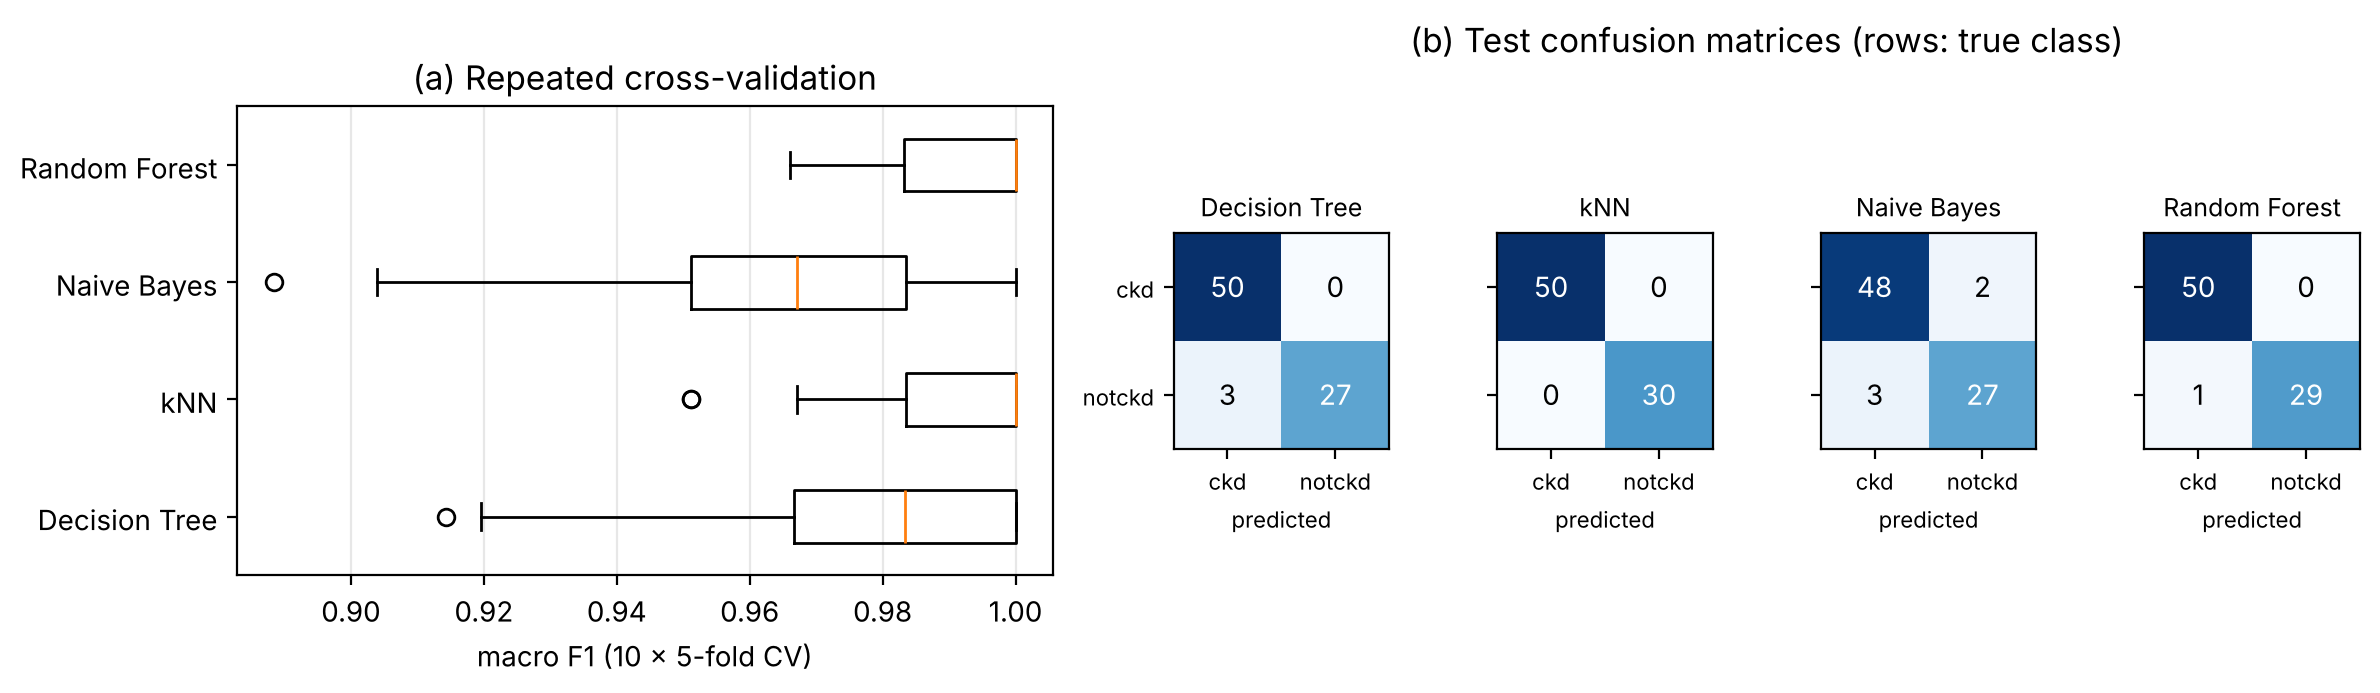
\includegraphics[width=\textwidth]{figures/classical_comparison.png}
\caption{(a) Macro F1 of the four final classical models across the same 50 cross-validation folds. (b) Confusion matrices on the 80 test patients.}
\label{fig:classical}
\end{figure}

kNN and Random Forest are tied in cross-validation, and the test set agrees with this ranking: they differ by one patient, while Naive Bayes trails kNN by five. Only Naive Bayes misses CKD patients on the test set. Within each model, the tuning steps changed less than expected. For the Decision Tree, the fully grown, grid-tuned and pruned trees scored within 0.006 of each other in repeated CV (0.973--0.979), well inside their spread. For Naive Bayes, tuning the smoothing had no effect up to $10^{-2}$, and the mixed Gaussian--Bernoulli model was worse (0.953) than plain Gaussian NB (0.961); only removing features helped (0.966). For kNN, feature selection was the largest gain (0.976 to 0.993). In two cases the test set reversed the cross-validation order within a model (the 30-feature Naive Bayes variants and the fully grown tree score higher on test than the chosen versions), by one to four patients; we kept the CV choice, since choosing on the test set would leak it into model selection.

The final tree (\fref{fig:tree}) uses only haemoglobin, specific gravity and albumin. These match the highest Random Forest importances (haemoglobin 0.328, specific gravity 0.157, red blood cell count 0.131) and the three features Naive Bayes kept, so all models rely on the same anaemia and urine-concentration markers.

\begin{figure}[H]
\centering
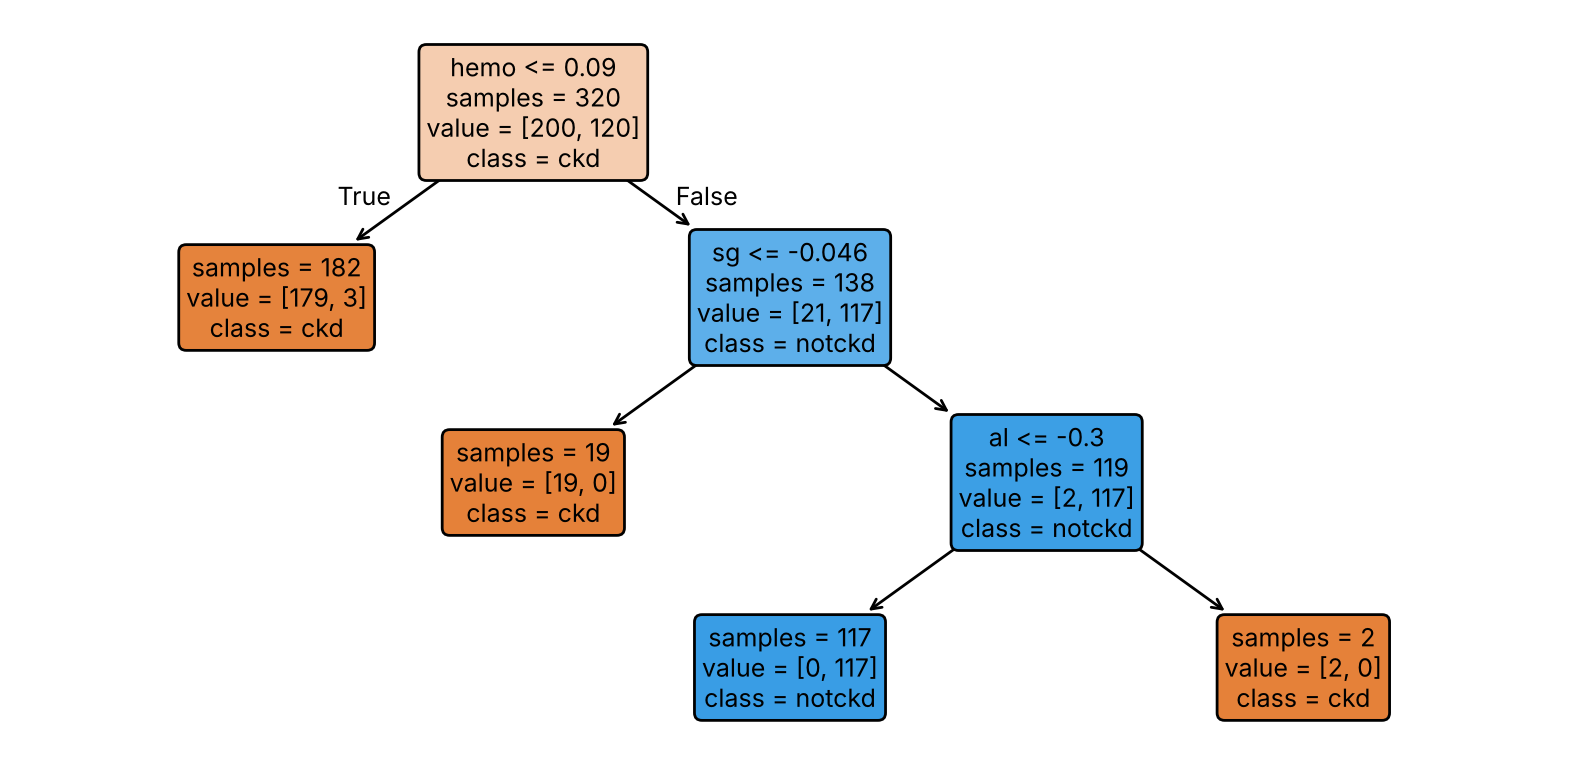
\includegraphics[width=0.62\textwidth]{figures/decision_tree.png}
\caption{Final pruned decision tree. Thresholds are on the standardised scale (0 = training mean).}
\label{fig:tree}
\end{figure}

\paragraph{Neural networks.}
\todo[5cm]{MLP and CNN scores, learning curves, comparison with the best classical model.}

\subsection{Further Analyses}
\todo[6cm]{Extra experiments and why.}
